\documentclass{article}
\usepackage{microtype}
\usepackage{graphicx}
\usepackage{booktabs}
\usepackage{multirow}
\usepackage{amsmath,amssymb,amsthm}
\usepackage{hyperref}
\usepackage{balance}
\usepackage[preprint]{icml2026}
\usepackage{algorithm}
\usepackage{algorithmic}
\graphicspath{{figures/}}
\newcommand{\ii}{\mathrm{i}}
\newcommand{\R}{\mathbb{R}}
\newcommand{\C}{\mathbb{C}}
\newcommand{\norm}[1]{\left\lVert#1\right\rVert}
\newcommand{\us}{u^{\mathrm{s}}}
\newcommand{\ut}{u^{\mathrm{tot}}}
\newcommand{\ui}{u^{\mathrm{i}}}
\newtheorem{proposition}{Proposition}
% No institutional affiliation or correspondence address was supplied for this
% preprint. Keep the official layout and use a notice-only author footnote.
% The vendored ICML style is unchanged; this affects only the author notice.
\makeatletter
\renewcommand{\printAffiliationsAndNotice}[1]{%
  \global\icml@noticeprintedtrue
  {\let\thefootnote\relax\footnotetext{\textit{Preprint. November 13, 2026.}}}}
\makeatother
\renewcommand{\today}{November 13, 2026}
\icmltitlerunning{Learning reduced scattering fields}
\hypersetup{pdftitle={Learning reduced scattering fields: representation limits and multiscale comparisons},pdfauthor={Egoriy Monastyrev}}

\begin{document}
\twocolumn[
\icmltitle{Learning Reduced Scattering Fields: Representation Limits and Multiscale Comparisons}
\begin{icmlauthorlist}
\icmlauthor{Egoriy Monastyrev}{}
\end{icmlauthorlist}
\icmlkeywords{Helmholtz scattering, reduced modeling, spectral neural operators, GMsFEM}
\vskip 0.3in
]
\printAffiliationsAndNotice{}
\hypersetup{pdfsubject={Research preprint; not a conference publication}}

\begin{abstract}
We study how spatial representation and coefficient prediction affect learned approximations of heterogeneous Helmholtz scattering. A coefficient-space spectral neural network predicts a complex field through separate train-fitted POD decoders for its real and imaginary parts, while a consistent finite element loss measures phase-sensitive error. On one fixed medium over $k\in[0.1,4]$, a shared model with 61 modes per component attains mean total-field error $2.366\%$ on 424 held-out queries; a prescribed GMsFEM configuration attains $3.244\%$, but has the lower median and is more accurate on most queries. The shared decoder's mean scattered-field projection floor is $0.1435\%$, well below its $3.327\%$ prediction error. A separate representation study identifies a coarse Chebyshev decoder as a limiting factor, whereas a frozen low-band surrogate fails outside its training range. These results support a diagnostic comparison of fixed-medium surrogates and multiscale reduction, with no claim of generalization to new materials or uniform superiority.
\end{abstract}

\section{Introduction}
Repeated scattering calculations require the wave field at several frequencies and incident directions. Fine finite element solutions resolve material interfaces but remain costly when many queries are needed. A reduced approximation stores spatial information in a smaller space. A physical reduced method then solves a projected equation, whereas a learned surrogate predicts the coefficients from data. The choice of space and the accuracy of this coefficient map are distinct sources of error.

We study this distinction for a two-dimensional Helmholtz problem. Our learned model uses proper orthogonal decomposition (POD) on an unstructured finite element mesh and a coefficient-space network adapted from spectral neural operators (SNO). The main dataset contains one fixed heterogeneous medium; only the wavenumber $k$ and incident direction $\theta$ vary. Thus the measured task is approximation of a parametric solution family. The architecture can accept material coefficients, but this experiment does not test an operator across different media.

The main comparison uses one network and one pair of output bases throughout $k\in[0.1,4]$. Four prescribed generalized multiscale finite element method (GMsFEM) configurations provide physical reduced approximations on the same held-out queries. We retain two further experiments because they test different failure mechanisms: a low-frequency comparison of POD, Fourier, and Chebyshev representations on another fixed medium, and a frozen low-band model evaluated at higher frequencies. Their datasets and denominators are kept separate.

The purpose is to make the approximation error interpretable. We give the actual decoder-space form of the consistent finite element loss, report the attainable projection error separately from the predictor error, and compare both means and paired query outcomes. The observed ordering changes with frequency and with the summary statistic. This is a numerical case study of existing reduced-modeling ideas, rather than a claim that combining POD and a neural coefficient map is a new principle.

\begin{figure*}[t]
\centering
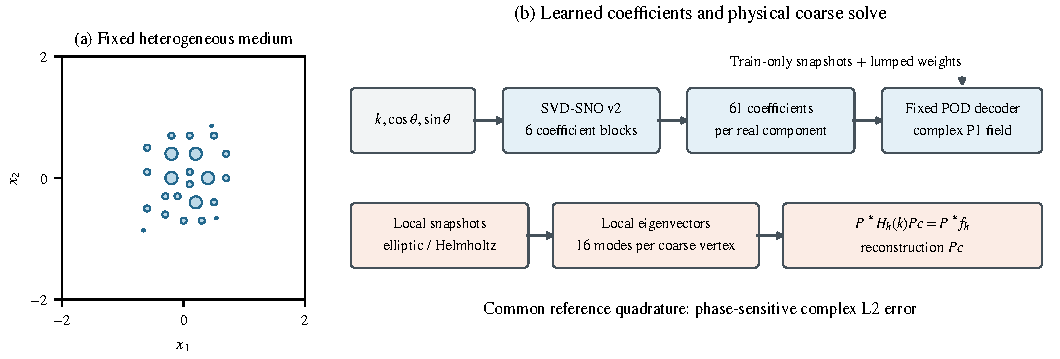
\includegraphics[width=\textwidth]{method.pdf}
\caption{The main experiment uses 24 penetrable circular inclusions in $\Omega=[-2,2]^2$, with $(\alpha,n)=(0.2,10)$ inside and $(1,1)$ outside. The learned route uses a shared output basis across the full wavenumber range; the physical route solves a projected Helmholtz system. POD ranks count global modes per real component, whereas GMsFEM retains local modes at each coarse vertex. These counts are not interchangeable.}
\label{fig:method}
\end{figure*}

\section{Related work}
GMsFEM constructs local approximation spaces through snapshot problems and spectral reduction, then couples them in a global coarse solve~\cite{efendiev2013}. For scattering in heterogeneous media, Kalachikova et al.~\cite{kalachikova2023} study elliptic and Helmholtz snapshot spaces. Our implementation follows that construction on the repository's saved geometry. It is an adaptation of the method, not a reproduction of the source article's tables.

Fourier neural operators learn kernels parameterized in Fourier space~\cite{li2021}. SNO instead learns maps between series coefficients, including Chebyshev and Fourier expansions~\cite{fanaskov2022}. Our SVD-SNO uses data-dependent spatial modes and a dense transformation of coefficient positions. These positions do not represent Fourier frequencies or eigenfunctions of the Helmholtz operator. The Chebyshev model is a separate implementation with its own tensor coefficient blocks.

Data-dependent output spaces also appear in POD-DeepONet~\cite{lu2022}. PODNO replaces Fourier transforms in an FNO-like construction by POD transforms~\cite{cheng2026}. Our network predicts coefficients in a fixed affine output space and is not an implementation of either architecture. These established methods motivate the use of representation diagnostics and limit the methodological novelty that can be inferred from our comparison.

\section{Scattering problem and discrete reference}
Let $\Omega=[-2,2]^2$, $\alpha(x)>0$, and $n(x)>0$. The material tensor is isotropic, $A(x)=\alpha(x)I$. With $d=(\cos\theta,\sin\theta)$, the incident and total fields are
\begin{equation}
\ui(x)=\exp(\ii k d\cdot x),\qquad \ut=\ui+\us.
\end{equation}
The total field satisfies
\begin{equation}
\nabla\cdot(\alpha\nabla\ut)+k^2n\ut=0.
\end{equation}
We approximate the exterior radiation condition by
\begin{equation}
\partial_\nu\us-\ii k\us=0\quad\text{on }\partial\Omega.
\end{equation}
All inclusions lie strictly inside $\Omega$, so $\alpha=n=1$ near its boundary. For a complex test function $v$, define
\begin{align}
a_k(u,v)&=\int_\Omega\alpha\nabla u\cdot\nabla\bar v
-k^2\int_\Omega nu\bar v\nonumber\\
&\hspace{1em}-\ii k\int_{\partial\Omega}u\bar v,\label{eq:weak}\\
F_{k,\theta}(v)&=\int_\Omega(1-\alpha)\nabla\ui\cdot\nabla\bar v\nonumber\\
&\hspace{1em}+k^2\int_\Omega(n-1)\ui\bar v.\label{eq:rhs}
\end{align}
The discrete scattered field satisfies $a_k(\us_h,v_h)=F_{k,\theta}(v_h)$ in a continuous complex P1 space. The weak contrast load in~\eqref{eq:rhs} retains the effect of discontinuous material interfaces; taking only cellwise derivatives of $\alpha$ would lose that contribution. In matrix form,
\begin{equation}
H_h(k)U_h=f_h,\quad H_h(k)=K_\alpha-k^2M_n-\ii k B.
\label{eq:fem}
\end{equation}

The main reference mesh has 53,246 nodes and 105,690 triangles, with nominal target size $h=0.02$. GMsFEM starts from a saved $h=0.04$ mesh with 17,549 nodes. The additional fine-FEM row measures the discrepancy of that mesh from the reference. A reference FEM solution still has discretization error and error from the artificial outer boundary.

For a P1 vector $U$ on one mesh, let $M$ be the consistent, unweighted mass matrix. The complex discrete norm is $\norm{U}_M^2=U^*MU$. We report samplewise relative errors
\begin{equation}
e^s=\frac{\norm{\widehat{\us}-\us_{\mathrm{ref}}}_{L^2}}
{\norm{\us_{\mathrm{ref}}}_{L^2}},\qquad
e^t=\frac{\norm{\widehat{\ut}-\ut_{\mathrm{ref}}}_{L^2}}
{\norm{\ut_{\mathrm{ref}}}_{L^2}}.
\label{eq:error}
\end{equation}
The incident wave is evaluated analytically for total-field comparisons. Adding the same incident wave leaves the complex error field unchanged but changes the relative denominator. Errors of $|u|$ alone do not measure phase error.

All main comparison fields are evaluated in the same reference-element quadrature. A source GMsFEM field is evaluated from its original P1 representation at those points, rather than first interpolated to reference nodes for scoring. This is a common evaluation protocol, not a proof of exact cross-mesh error integration. Exact integration on one P1 mesh applies to the neural decoder loss below.

\section{Reduced representations and learned map}
\subsection{Train-fitted spatial bases}
For each real field component, form the centered training snapshot matrix $X_c$. Let
\begin{equation}
W=\operatorname{diag}(M\mathbf{1}),\qquad
X_cW^{1/2}\approx U\Sigma V^T.
\end{equation}
We use the randomized range-finding construction of Halko et al.~\cite{halko2011}, with ten additional vectors and two power iterations. With $r$ retained right singular vectors,
\begin{equation}
\Phi=W^{-1/2}V_r,\qquad \Phi^TW\Phi=I.
\label{eq:pod}
\end{equation}
The encoder of a centered field is $a_W=\Phi^TW(u-\mu)$, and the decoder is $\mu+\Phi a$. Separate means and bases are fitted to real and imaginary components. This is lumped-weight POD, not POD optimized in the consistent $M$ norm.

All bases, coefficient statistics, and wavenumber statistics use training data. The common rank is the smallest available rank whose mean validation reconstruction error is at most $0.1\%$, subject to a cap of 96. That reconstruction uses the lumped-weight encoder and is scored in the consistent FEM norm. The selected rank is 61 for both real components. The material is constant over samples, so centered input material ranks are both zero.

\subsection{Coefficient-space network}
In the general implementation, token $j$ contains
\begin{equation}
t_j=(\widetilde a_{\alpha,j},\widetilde a_{n,j},
\cos\theta,\sin\theta,\widetilde k).
\end{equation}
The two material sequences are padded independently, without identifying their bases with the solution bases. In this fixed-medium experiment they are zero. Wavenumber normalization is shared across $[0.1,4]$ and fitted on train. A five-channel affine lift and GELU produce a feature table $Z\in\R^{r\times w}$. Each of six blocks computes
\begin{equation}
Z^{\ell+1}=Z^\ell+\operatorname{GELU}\!\left(
Z^\ell W^\ell_{\mathrm{loc}}+b^\ell
+B^\ell Z^\ell W^\ell_{\mathrm{ch}}\right).
\label{eq:block}
\end{equation}
Here $B^\ell$ mixes coefficient positions, while the two $W$ matrices act on channels. A shared head returns two normalized coefficients per position. After train-statistic denormalization,
\begin{equation}
\widehat{\us}=\mu_R+\Phi_R\widehat a_R
+\ii(\mu_I+\Phi_I\widehat a_I).
\label{eq:decode}
\end{equation}
With width 48 and rank 61 the network has 50,648 trainable real scalars. This count excludes the stored spatial bases. No frequency routing or query-specific decoder is used.

\subsection{Consistent FEM loss in coefficient coordinates}
The lumped POD encoder does not give the best consistent-mass projection. For component $c\in\{R,I\}$, define
\begin{align}
G_c&=\Phi_c^TM\Phi_c,\nonumber\\
a_c^\star&=G_c^{-1}\Phi_c^TM(u_c-\mu_c),\label{eq:best}\\
\rho_c&=u_c-\mu_c-\Phi_ca_c^\star.\nonumber
\end{align}
Since $\Phi_c^TM\rho_c=0$, the discrete squared error satisfies
\begin{align}
\norm{\widehat u-u}_M^2
&=\sum_{c\in\{R,I\}}
(\widehat a_c-a_c^\star)^TG_c(\widehat a_c-a_c^\star)\nonumber\\
&\hspace{1em}+\sum_{c\in\{R,I\}}\norm{\rho_c}_M^2.\label{eq:identity}
\end{align}
We minimize the arithmetic mean of the square root of~\eqref{eq:identity} divided by the reference scattered-field norm. The Gram matrices, best projection coefficients, residual energies, and reference norms are precomputed. Residual energies are integrated directly, avoiding cancellation from subtracting nearly equal total and projected energies. Online loss evaluation depends on the rank rather than the number of mesh nodes.

The mean of $\sqrt{\sum_c\norm{\rho_c}_M^2}/\norm{u}_M$ is the attainable error floor of this fixed affine decoder. It is a representation diagnostic with access to the target field, not a deployable predictor. Identity~\eqref{eq:identity} holds samplewise for squared errors. Subtracting two reported mean relative errors does not isolate coefficient prediction error. We construct these quantities from the actual rounded decoder buffers; the implementation details and a direct numerical check are given in Appendix~\ref{app:loss}.

\subsection{GMsFEM comparison}
For each coarse-vertex patch, local boundary delta data are extended by the elliptic operator (type 1) or by the Helmholtz operator (type 2). In the snapshot space $\Psi_p$, the local eigenproblem is
\begin{equation}
\Psi_p^*K_{\alpha,p}\Psi_p z
=\lambda\Psi_p^*S_{\alpha,p}\Psi_p z,
\end{equation}
where $S_{\alpha,p}$ is the local mass matrix weighted by $\alpha$. The stiffness in this eigenproblem remains elliptic for both snapshot types. The 16 eigenvectors with the smallest eigenvalues are multiplied by continuous coarse-vertex functions, whose local extensions use the corresponding operator. Their global columns form $P$. The coarse solution is
\begin{equation}
(P^*H_h(k)P)c=P^*f_h,\qquad U_{\mathrm{ms}}=Pc.
\end{equation}
The two coarse grids, $10\times10$ and $20\times20$, give 1,936 and 7,056 unknowns. Type 2 construction depends on $k$. A small coarse-system residual checks its algebraic solution, not closeness to the reference field.

\section{Experimental protocol}
The main study combines 2,568 existing reference fields at 320 distinct wavenumbers. The grid is the union of the earlier low- and high-band query grids, not a new uniform discretization. Eight directions occur at each frequency except $k=2$, where the union contains 16 distinct directions. The physical frequency group is kept intact across splits, including this shared endpoint. There are 1,712/432/424 train/validation/test fields at 214/54/52 frequencies. Endpoints and the anchor $k=1$ were reserved as test queries in the original protocol. Interior held-out frequencies probe interpolation; endpoints also test the boundary of the sampled range.

AdamW uses initial learning rate $0.002$, weight decay $10^{-5}$, batch size 32, gradient clipping at 1, and seed 42. A validation-driven scheduler halves the learning rate after 20 plateau epochs, with minimum $10^{-5}$. The run reaches its limit of 500 epochs; checkpoint 493 is selected by validation. Reaching this limit is not evidence that optimization has converged. Rank and checkpoint selection do not use test scores. More detail is in Appendix~\ref{app:protocol}.

All four GMsFEM configurations are retained. Their per-query records are imported from the verified earlier experiments by exact source identity, $k$, and $\theta$, with label and geometry checksums. The archived verification additionally recomputed the fine FEM and $20\times20$ type 2 GMsFEM at four anchor frequencies. We reloaded every shared neural test prediction during this revision and checked the source and checkpoint hashes. The fresh checks are distinguished from archived FEM checks in Appendix~\ref{app:checks}.

We report arithmetic means, medians, 95th percentiles, and maxima of samplewise relative norms. The eight directions within a frequency group are related observations; the 424 fields are not 424 independent frequency samples. No confidence interval over media or variation across training seeds is estimated. Parameter counts, coarse unknown counts, and hardware timings answer different cost questions and are not treated as an equal-budget comparison.

\begin{table*}[t]
\caption{Main fixed-medium comparison on the same 424 test queries, with reference FEM $h=0.02$. All errors are percentages of the corresponding complex reference-field norm. The size column gives trainable network scalars for SNO and algebraic unknowns for the physical methods; the units are intentionally distinguished. Every GMsFEM configuration uses 16 local modes per coarse vertex and starts from the $h=0.04$ fine mesh.}
\label{tab:main}
\centering\small
\setlength{\tabcolsep}{4pt}
\begin{tabular}{llrrrrrr}
\toprule
& & \multicolumn{4}{c}{Total field} & \multicolumn{2}{c}{Scattered field}\\
\cmidrule(lr){3-6}\cmidrule(lr){7-8}
Method & Size & Mean & Median & p95 & Max & Mean & p95\\
\midrule
Shared SVD-SNO & 50,648 weights & 2.366 & 1.332 & 7.372 & 27.586 & 3.327 & 9.373 \\
FEM ($h=0.04$) & 17,549 & 0.532 & 0.285 & 1.770 & 4.052 & 0.708 & 2.236 \\
GMsFEM $10\times10$, type 1 & 1,936 & 19.597 & 10.135 & 59.148 & 78.843 & 26.214 & 80.369 \\
GMsFEM $10\times10$, type 2 & 1,936 & 12.213 & 3.696 & 68.952 & 118.750 & 16.129 & 87.125 \\
GMsFEM $20\times20$, type 1 & 7,056 & 12.568 & 5.902 & 39.497 & 72.523 & 16.622 & 52.178 \\
GMsFEM $20\times20$, type 2 & 7,056 & 3.244 & 1.185 & 12.662 & 30.801 & 4.293 & 15.648 \\
\bottomrule

\end{tabular}
\end{table*}

\begin{figure*}[t]
\centering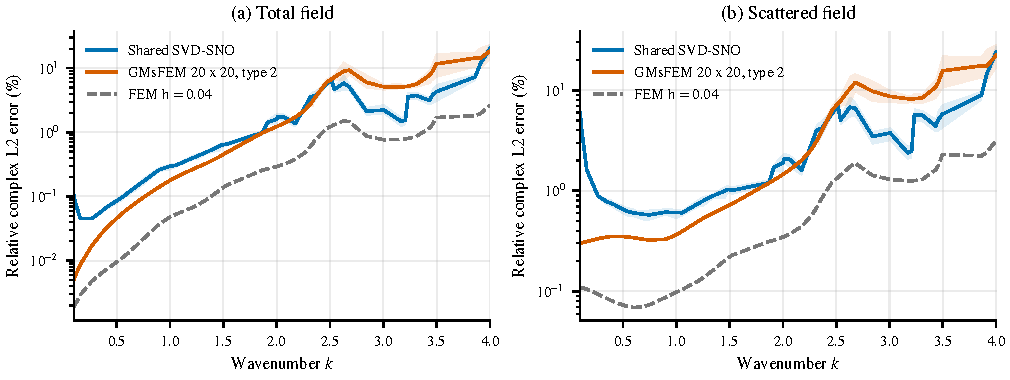
\includegraphics[width=\textwidth]{frequency_errors.pdf}
\caption{Error versus wavenumber in the main experiment. Lines join the mean over directions at each of the 52 held-out physical frequencies; shaded bands show directional 10th--90th percentiles, not confidence intervals. The displayed GMsFEM is the $20\times20$ type 2 setting. The $h=0.04$ FEM discrepancy is shown separately. Total- and scattered-field denominators differ.}
\label{fig:frequency}
\end{figure*}

\section{Results}
\subsection{The ordering depends on frequency and statistic}
Table~\ref{tab:main} reports mean total-field errors of $2.3656\%$ for shared SVD-SNO and $3.2439\%$ for the most accurate of the four saved GMsFEM settings by this mean. The corresponding scattered-field means are $3.3271\%$ and $4.2925\%$. The $h=0.04$ fine FEM has mean total error $0.5322\%$, showing the baseline mesh discrepancy without multiscale reduction. Thus the two reduced methods are not approximating exactly the same finite-dimensional reference system.

The lower SNO mean does not imply typical-query dominance. GMsFEM has the lower total-field median, $1.1848\%$ versus $1.3316\%$, and lower error on 285 of the 424 paired queries. SNO has lower error on 139. Its total-field p95 is $7.3718\%$ and its maximum is $27.5856\%$. Figure~\ref{fig:distributions} displays both the cumulative distribution and the paired outcomes, so that a change in the tail cannot be mistaken for a uniform improvement.

The interval summaries agree with this pattern. For $k\in[0.1,1]$, total-field means are $0.1125\%$ for SNO and $0.0545\%$ for GMsFEM; for $k\in(1,2]$, they are $0.7970\%$ and $0.5998\%$. In $(2,3]$ the ordering reverses, at $3.6470\%$ and $4.4610\%$, and in $(3,4]$ the means are $5.7229\%$ and $9.2187\%$. These intervals describe one shared model, not separate networks. Figure~\ref{fig:frequency} shows the frequency dependence without fitting a smooth trend through the errors.

\begin{figure*}[t]
\centering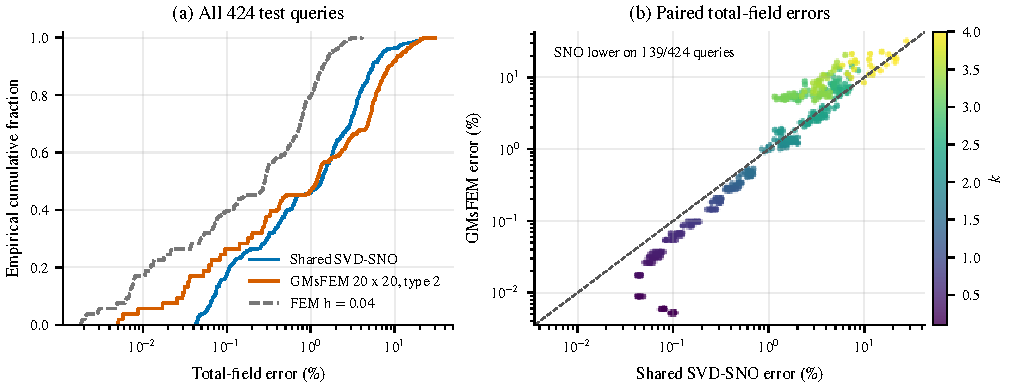
\includegraphics[width=\textwidth]{error_distributions.pdf}
\caption{The mean comparison does not describe most individual queries. Left: empirical cumulative distributions of total-field errors. Right: exact query pairs for shared SNO and $20\times20$ type 2 GMsFEM, colored by $k$; points above the diagonal favor SNO. SNO has lower error on 139 queries, while GMsFEM has the smaller median. All points are shown.}
\label{fig:distributions}
\end{figure*}

\subsection{Representation capacity does not explain the shared prediction gap}
The shared affine decoder has mean consistent-mass test floor $0.1435\%$ for the scattered field. Its learned prediction error is $3.3271\%$. Hence the chosen span admits much more accurate fields than the present coefficient map predicts. This observation identifies where the error can be reduced, but not its cause: optimization, training coverage, scaling, and network design have not been separated by controlled ablations. Adding more POD modes alone is not supported as the first remedy by these data.

Figure~\ref{fig:fields} shows the real scattered field and absolute complex differences at the fixed verification anchors $k=1$ and $k=4$. These examples were not chosen by minimizing either model's error. Fields use shared color limits within each row. GMsFEM is transferred to reference nodes for display only; its reported scores use its original P1 evaluation at reference quadrature points. Spatial images and integrated scores therefore have explicitly different evaluation purposes.

\begin{figure*}[t]
\centering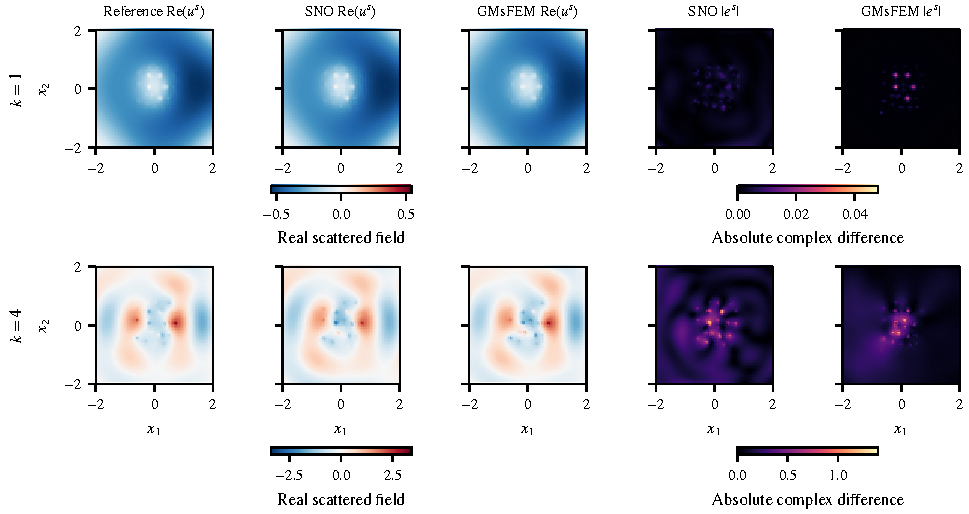
\includegraphics[width=\textwidth]{field_examples.pdf}
\caption{Two predetermined verification examples from the main test set: $k=1$ and $k=4$. The first three columns show the real scattered field; the last two show the magnitude of the complex difference from the reference. Color scales are common across methods within each quantity and row. The GMsFEM setting is $20\times20$, type 2, with 16 local modes. The reference and predicted fields are P1 visualizations, not independently generated illustrations.}
\label{fig:fields}
\end{figure*}

\subsection{A separate representation study}
The static-low dataset contains 8,000 fields on a 3,221-node mesh, with $k\in[1,2]$ and eight directions at each of 1,000 frequencies. Its geometry and material contrasts differ from the main study. The split is 5,360/1,360/1,280 fields by complete frequency groups. All three architectures use the same fields and consistent FEM scoring; their capacities and devices differ. We use this dataset to examine the output representation, without pooling its errors with Table~\ref{tab:main}.

SVD-SNO uses ten POD modes per component and has mean test error $0.9475\%$, close to its $0.9188\%$ consistent-decoder floor. FNO and Chebyshev-SNO have means $1.6599\%$ and $7.9364\%$. At the retained $8\times8$ Chebyshev modes on a $32\times32$ Lobatto grid, the best consistent-mass projection into the actual affine decoder span has mean validation error $7.6143\%$. Increasing to 12 or 16 modes per axis lowers this validation floor to $5.8905\%$ or $4.7016\%$ (Figure~\ref{fig:representation}). These are target-assisted projections with no neural training. They show a limitation of the chosen polynomial span, not a defect in the DCT-I transform or the best accuracy attainable by the Chebyshev architecture. The validation floors are not subtracted from test errors.

\begin{figure*}[t]
\centering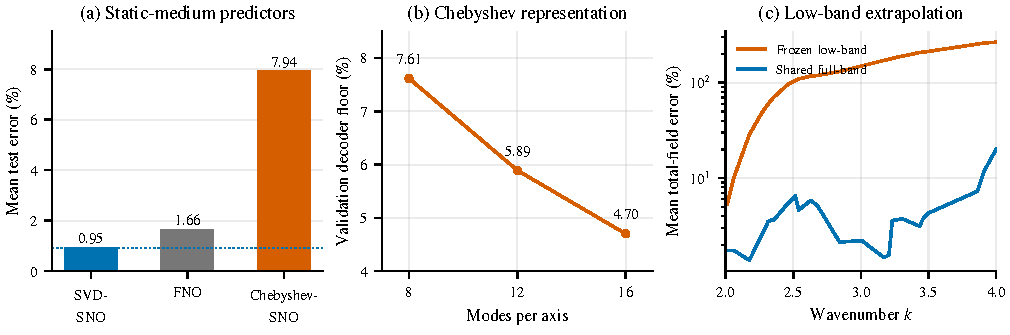
\includegraphics[width=\textwidth]{diagnostics.pdf}
\caption{Representation and frequency-coverage diagnostics. Left: separate static-medium test errors for three architectures; the dotted line is the POD test floor. Center: validation-only best projections into Chebyshev spans on a $32\times32$ grid. These two panels use different splits and do not define a numerical learning gap. Right: the frozen low-band model and the shared full-band model on the same 200 queries with $k>2$; lines show directional means of total-field error. The full-band model is not extrapolating. Model sizes appear in Table~\ref{tab:static}.}
\label{fig:representation}
\label{fig:ood}
\end{figure*}

\subsection{Training-range coverage is essential in the saved extrapolation test}
A separate SNO trained on $k\in[0.1,2]$ was frozen and tested on 200 held-out queries with $k>2$. Its mean total-field error is $131.8231\%$, and its mean scattered-field error is $177.7174\%$. The low-band basis, weights, and wavenumber normalization remain fixed. On these exact same 200 physical queries, the shared full-band SNO has mean total error $4.5604\%$. The latter has been trained throughout the declared range and is not an extrapolating model.

Figure~\ref{fig:ood} retains this failure. Because the two networks have different training ranges and bases, it is not an ablation of one isolated architectural choice. It establishes failure of the particular frozen low-band surrogate; it does not prove that the shared network will generalize beyond $k=4$.

\section{Limitations}
Both completed datasets use one fixed material realization each. Holding out frequencies avoids overlap at the same physical $k$, but does not test a new medium, a new mesh, or a different boundary model. One training seed gives no estimate of variation across optimization runs. A matched POD-MLP baseline would be needed to establish whether the particular coefficient mixer improves on a simpler map with the same decoder. No such result is claimed here.

The reference is a discrete P1 solution, and the first-order absorbing condition is an approximation of the exterior problem. Fine-mesh refinement and outer-boundary studies are required to estimate continuum error. GMsFEM begins on a different fine mesh, and the common cross-mesh quadrature has not been subjected to a convergence study. Consequently, the baseline discrepancy combines reduction, discretization, and possible integration effects. It is not a pure reduction error measured in one common discrete space.

The architectures and physical methods have different stored spaces, training requirements, and computational budgets. The network weight count excludes POD modes, means, and mesh information. Existing timing records mix computational contexts and include different transfer work. We therefore make no end-to-end acceleration claim. Such a measurement must include supervised label generation, POD preprocessing, training, frequency-dependent multiscale setup, and clearly defined online workloads.

\section{Conclusion}
A useful comparison of learned and physical reduced models must distinguish spatial representation from coefficient prediction. In the shared fixed-medium study, the POD span is considerably more accurate than its learned predictor, while the separate coarse Chebyshev representation itself limits reconstruction. The shared SNO has the lower mean than the best recorded GMsFEM setting, but GMsFEM has the smaller median and is more accurate on most queries. The frozen low-band failure further limits the interpretation of interpolation results. These conclusions concern the specified scattering families and provide a reproducible basis for subsequent controlled experiments.

\section*{Impact statement}
This work concerns numerical approximations of wave scattering. Its direct contribution is a reproducible computational case study. The reported errors do not certify accuracy for safety-critical simulation or for untested materials and frequencies. Reusing verified data and retaining failed predictions can reduce wasted computation and discourage unsupported reliability claims.

\clearpage
\raggedbottom
\balance
\bibliography{references}
\bibliographystyle{icml2026}

\clearpage
\nobalance
\appendix
\onecolumn
\section{Discrete decoder loss and numerical precision}\label{app:loss}
For a real component, write $v=u-\mu$ and $G=\Phi^TM\Phi$. Assuming that the retained columns are linearly independent, $G$ is positive definite. The minimizer of $\norm{v-\Phi a}_M^2$ is $a^\star=G^{-1}\Phi^TMv$. Setting $\rho=v-\Phi a^\star$ gives $\Phi^TM\rho=0$, hence
\begin{equation}
\norm{\Phi\widehat a-v}_M^2
=\norm{\Phi(\widehat a-a^\star)-\rho}_M^2
=(\widehat a-a^\star)^TG(\widehat a-a^\star)+\rho^TM\rho.
\end{equation}
Real and imaginary component energies add because $M$ is real symmetric. This proves~\eqref{eq:identity}. The identity does not require $\Phi^TM\Phi=I$. Replacing $G$ by the identity, or replacing $a^\star$ by the lumped encoder $\Phi^TWv$, would generally change the loss.

The implementation first rounds means and modes to the float32 decoder representation, then builds $G$, $a^\star$, and residual energies in float64. Targets are rounded to the component precision used during training. Denormalization follows the decoder's float32 operations before the quadratic form is evaluated. A direct comparison on 12 fixed test queries during this revision gives mean relative loss $0.0436051287351$ from the reduced form and $0.0436051277424$ from decoded P1 fields, an absolute difference of $9.93\times10^{-10}$. The identity is exact for the specified discrete vectors in exact arithmetic; the implementation agreement is numerical.

For zero or extremely small squared errors, the training routine uses a bounded-gradient continuation: the numerator norm is $e/\sqrt{\max(e,\varepsilon)}$, with $e$ a nonnegative squared error and $\varepsilon=10^{-24}$. The reference squared norm is also bounded below by $\varepsilon$. This yields exactly zero for a perfect zero field and agrees with the ordinary square root away from the tiny threshold. It is not used to interpret near-zero fields as relative physical accuracy.

\section{Training and data details}\label{app:protocol}
\begin{table}[h]
\centering
\caption{Shared-model configuration. All quantities describe the completed saved run.}
\begin{tabular}{ll@{\hspace{2em}}ll}
\toprule
Quantity & Value & Quantity & Value\\
\midrule
Medium count & 1 & Wavenumber range & $[0.1,4]$\\
Train/validation/test fields & 1712/432/424 & Frequency groups & 214/54/52\\
Reference nodes/triangles & 53,246/105,690 & POD rank per component & 61\\
Material ranks & 0, 0 & Rank cap / validation target & 96 / $0.1\%$\\
Coefficient width / depth & 48 / 6 & Trainable real scalars & 50,648\\
Optimizer & AdamW & Initial learning rate & $0.002$\\
Weight decay & $10^{-5}$ & Batch size & 32\\
Gradient clipping & 1 & Seed & 42\\
Completed / selected epoch & 500 / 493 & Stopping reason & Epoch limit\\
Scheduler factor / patience & 0.5 / 20 & Minimum learning rate & $10^{-5}$\\
CPU threads & 2 & Final learning rate & $6.25\times10^{-5}$\\
\bottomrule
\end{tabular}
\end{table}
The saved run reports 170.61 seconds of preprocessing and 634.51 seconds of training. These are descriptive run records, not isolated hardware benchmarks or total costs of obtaining a surrogate. No reported physical model was retrained for this manuscript. Training curves are shown in Figure~\ref{fig:training}. The learning rate is the rate actually used in an epoch; the scheduler steps after validation.

The main network stores two $53{,}246\times61$ decoder matrices, two field means, and mesh data in addition to its trainable scalars. For float32 modes alone, the storage is $2\cdot53{,}246\cdot61\cdot4=25{,}984{,}048$ bytes (about 24.8 MiB). Describing the complete predictor only by its 50,648 trainable weights would omit most of this spatial storage. The general bundle also preserves preprocessing needed for physical inference.

The static-low study uses a fixed medium drawn under the saved coefficient ranges $\alpha_{\mathrm{in}}\in[0.6,0.9]$ and $n_{\mathrm{in}}\in[1.5,3]$, with 3--10 active candidates from the geometry's 24 circles. The realized medium is shared by all 8,000 queries, not resampled for each field. Its nominal target mesh size is $h=0.1$. The three models use width 24 and depth 3; FNO and Chebyshev use grid resolution 32 with eight retained modes per axis. SVD-SNO and Chebyshev were trained in the recorded revision; the FNO checkpoint was independently rechecked. Device and capacity differences prevent interpreting the table as an equal-budget architecture study.

\begin{table}[h]
\centering
\caption{Separate static-low experiment: 1,280 held-out fields, scattered-field consistent FEM errors in percent. The final column distinguishes completed epochs from the validation-selected epoch.}
\label{tab:static}
\begin{tabular}{lrrrr}
\toprule
Method & Trainable real scalars & Mean & p95 & Completed / selected epoch\\
\midrule
SVD-SNO v2 & 4,022 & 0.9475 & 1.6534 & 165/115 \\
FNO & 445,010 & 1.6599 & 1.9505 & 142/92 \\
Chebyshev-SNO & 2,426 & 7.9364 & 9.8811 & 200/199 \\
\bottomrule

\end{tabular}
\end{table}

\begin{figure}[t]
\centering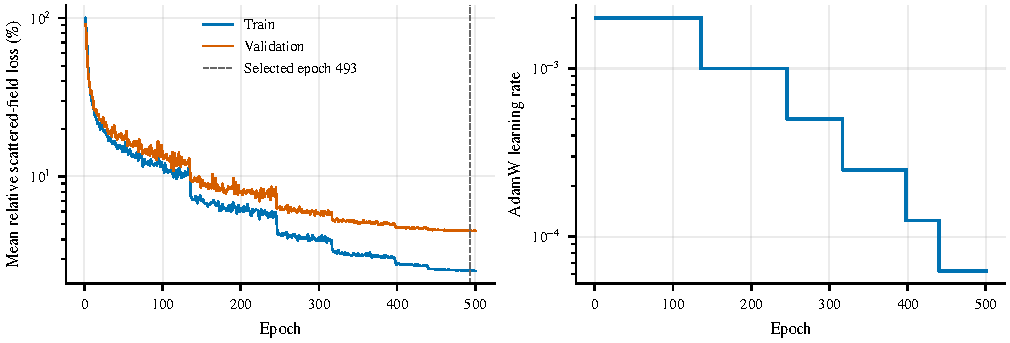
\includegraphics[width=.88\textwidth]{training.pdf}
\caption{The saved shared-model training history: scattered-field consistent loss and validation-driven learning rate. The selected checkpoint is epoch 493. Train values average batch losses while parameters change within an epoch; validation uses a fixed epoch-end model. Their curves need not be ordered at every epoch.}
\label{fig:training}
\end{figure}

\section{Chebyshev transform and affine decoder}
On ascending Lobatto nodes $x_j=-\cos(\pi j/(N-1))$, $j=0,\ldots,N-1$, define $S_{jm}=T_m(x_j)$ and $D=\operatorname{diag}(1/2,1,\ldots,1,1/2)$. The implemented analysis matrix is
\begin{equation}
A=\frac{2}{N-1}D S^T D,\qquad AS=I.
\end{equation}
Coefficients use $f(x)=\sum_m a_mT_m(x)$ with no implicit endpoint half-factors. Analysis and synthesis are applied along each tensor axis. The neural map acts on the truncated coefficient table, with GELU in coefficient space. Synthesis returns values on the same grid; bilinear transfer maps these values to the original FEM nodes, followed by the saved field mean and component scaling.

The relevant floor is therefore the best consistent-mass projection into the actual affine FEM-node decoder span, including grid synthesis, transfer, and the train-fitted mean. It is not merely a spectral truncation error evaluated on Lobatto nodes. The reported 8/12/16-mode floors use 1,360 validation targets, with no test-based rank search and no fitted neural weights. Their Gram condition numbers are approximately 102.0, 130.6, and 227.8. Fresh float64 checks of $AS=I$ for $N=2,9,16,32$ have maximum entrywise error $2.23\times10^{-15}$. This confirms transform normalization at those sizes, not a general error estimate for nonsmooth fields.

\section{Evidence and reproducibility}\label{app:checks}
The accompanying source tree includes the manuscript, official unmodified ICML 2026 style files in preprint mode, figure-generation code, paper-local score snapshots, field examples, and a source-hash manifest. All eight figure pairs are exported as PDF and PNG, including individual and combined diagnostic panels. Plots use numerical records; the method diagram is an original programmatic drawing. No synthetic observation is used as experimental evidence. The earlier manuscript and existing data, weights, and reports are preserved.

Fresh checks in this revision include 91 targeted numerical tests (plus two subtests), disjointness of the physical frequency sets, source and label hashes, reconstruction of all 424 shared test predictions, an explicit loss-identity comparison on 12 fixed queries, and the four Chebyshev inverse checks above. The maximum relative difference between fresh and archived shared predictions is $3.36\times10^{-6}$ in the consistent norm. The maximum difference in scattered-field error is $7.56\times10^{-5}$ percentage points. The fresh environment uses PyTorch 2.15.0 and NumPy 2.5.4; the original shared training record uses PyTorch 2.9.1+cpu and NumPy 2.4.6. Small floating-point differences are retained in the audit rather than presented as exact bitwise reproduction.

Archived verification reports additionally document independent FEM and GMsFEM recalculation at $k=0.1,1,2,4$, with maximum metric discrepancy $2.64\times10^{-12}$ percentage points from the stored baseline records. These PDE solves were not rerun in this manuscript revision. There was no new FEM-label generation, and none of the reported physical models was retrained. This distinction is part of the evidence ledger.

The scripts regenerate tables directly from per-query records and verify their summary values. The two physical display examples are the existing verification anchors at $k=1$ and $k=4$, rather than examples selected by a favorable test score. The paired extrapolation plot matches exact $(k,\theta)$ identities on all 200 out-of-range low-band queries. This produces the derived full-band mean $4.5604\%$ on that same subset; it should not be confused with the main full-test mean $2.3656\%$.

The present evidence does not establish new-material generalization, mesh-independent prediction accuracy, continuum PDE convergence, cross-mesh quadrature convergence, multi-seed robustness, or a cost-normalized advantage. These require further experiments. A direct coefficient regressor with the same POD decoder, multiple media and seeds, and controlled total-cost measurements would address distinct unresolved questions.
\end{document}
